\section{Background}
\subsection{Sokoban}
Sokoban is a single-player transport puzzle game where the player pushes boxes around into predetermined locations. A level is completed when all boxes are pushed into the correct spots. The player can move and push boxes in 4 directions: up, down, left and right, and is contained by walls surrounding the level. \autoref{fig:sokoban} shows an example of a simple Sokoban level. Not only is solving Sokoban puzzles NP-hard, but it is also proven to be PSPACE-complete\cite{pspace-complete}, making it significantly more difficult to solve than many other NP-hard problems. As a result, there exist many levels that state-of-the-art solvers cannot solve. 

\begin{figure}[h]
    \centering
    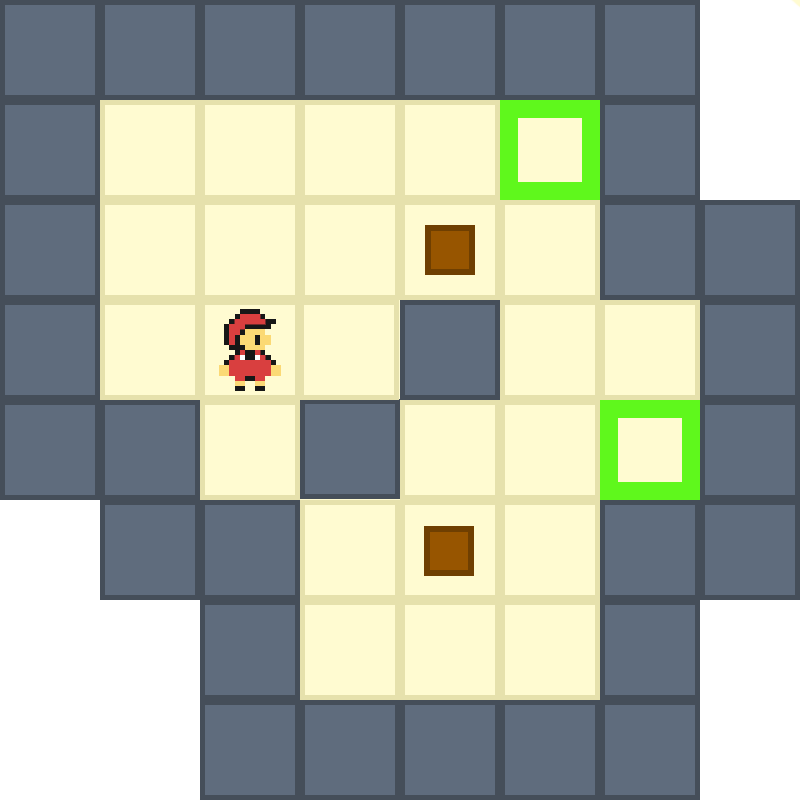
\includegraphics[width=5cm]{sokoban}
    \caption{An example Sokoban level. The gray tiles represent walls, the brown tiles represent boxes, and the green tiles are the targets.}
    \label{fig:sokoban}
\end{figure}

\subsection{Probabilistic model checking}
Model checking is a way of verifying the correctness of requirements of models. These models are often represented as finite-state machines. Using model checking tools, one can run queries on these state machines to verify the correctness of certain aspects of the model. A model of a Sokoban level would include the player and box positions, and the solution can be found by querying a state where all boxes are in the solved position. Probabilistic model checking is a similar technique that allows for verifying properties of models that exhibit stochastic behaviour. An example of such a model would be the model of a Sokoban level, but all inputs are randomly determined. One can now query the probability that the model ends up in an unsolvable state (e.g a box is pushed in a corner and can no longer move) or what the average length is to complete the level.

\subsection{Sok format}
.sok files\footnote{\url{http://www.sokobano.de/wiki/index.php?title=Sok_format}} are files that contain Sokoban levels. There are currently tens of thousands of user-created levels in this format freely available online. Apart from a few inconsistencies, the format is easy to parse and the large selection of levels makes it a good choice for this research. The contents of a .sok-file is depicted in \autoref{fig:sok}.

\lstset{basicstyle=\footnotesize\ttfamily,breaklines=true}

\begin{figure}[h]
    \subfloat[\centering ASCII representation of a .sok-file. '@' represents the player, '\$' represents a box, '.' represents a target location, and '\#' represents a wall.\label{fig:sok_ascii}]{\makebox[0.5\linewidth][c]{\lstinputlisting{code/level.sok}}}
    \hfill
    \subfloat[\centering Graphical representation of a .sok-file. The brown tiles represent boxes, the green tiles represent target locations, and the tiles blocks represent walls.]{\makebox[0.5\linewidth][c]{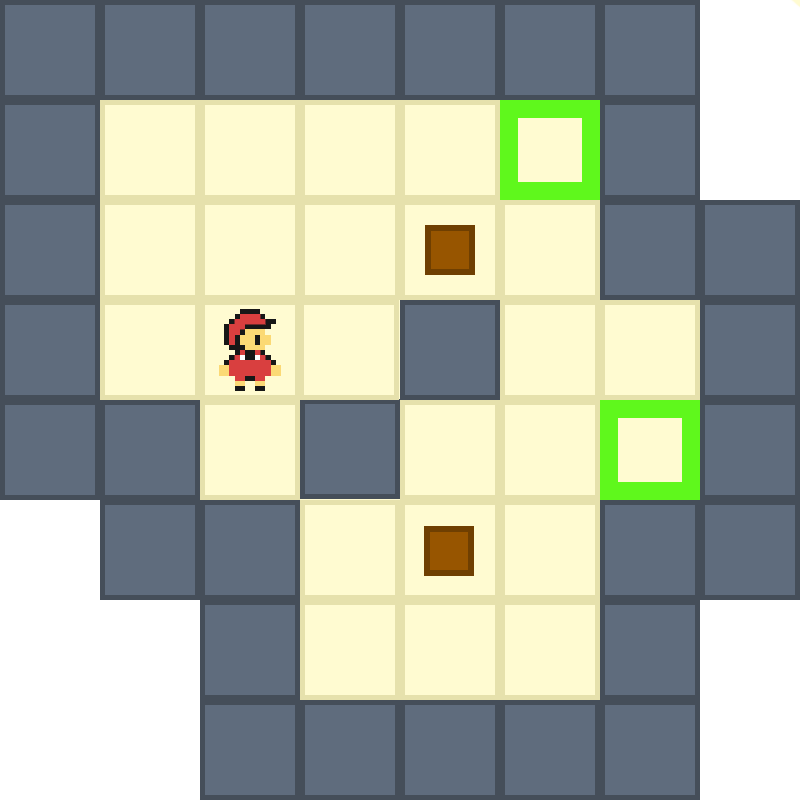
\includegraphics[width=3.5cm,valign=c]{sokoban.png}}}
    \caption{A .sok-file in both its ASCII and graphical representation.}
    \label{fig:sok}
\end{figure}
